\chapter{压缩后缀数组的实现}

\section{后缀数组和压缩后缀数组}
压缩后缀数组(CSA)是由Grossi和Vitter\cite{grossi2005compressed}最早提出的第一种实现全文索引的压缩索引数据结构,是对后缀数组(SA)
\cite{manber1993suffix}占用空间过大的改进,并且实现了自索引特性。

设长为$n$的文本序列$T$,字符集为$\Sigma$,本文中将假设$T$有一个特殊的结尾符号$\$$,$\$$不在$\Sigma$中并且字典序小于$\Sigma$
中的所有符号。假设$T$存储在一个数组$T[0\ldots n-1]$中。对任何的整数$i$,假设
\begin{itemize}
    \item $T[i]$为$T$中从左往右0开始的第$i$个字符;
    \item $T_i$为$T$的第$i$个后缀,即$T_i=T[i]T[i+1]\ldots T[n-1]$。
\end{itemize}

$T$的后缀数组$SA[0\ldots n-1]$定义为
$T$的$n$个后缀按字典序排序后的序列,由$\{0,1,\ldots, n-1\}$的一个排列构成,满足$T_{SA[0]}<T_{SA[1]}<\ldots<T_{SA[n-1]}$。即$SA[i]$
表示$T$的$n$个后缀中第$i$小的后缀的开始位置。如表\ref{tab:tabsuffix}所示。后缀数组占用空间$n\log n$,给定文本$T$和其后缀数组
$SA[0\ldots n-1]$,$T$中的任何模式$P$可以在$O(|p|\log n+occ)$时间复杂度内求出其出现位置\cite{manber1993suffix},并且不需要
读原文本$T$。其中$occ$是模式的出现次数。

对于任意的整数$i \in [0\ldots n-1]$,定义$SA^{-1}[i]=j$使得$SA[j]=i$,很明显$SA^{-1}[i]$为$T_i$在$T$的所有后缀中的排名,即
$T$的后缀中比$T_i$小的后缀的数量。

\begin{table}[htbp]
    \caption{$acaaccg\$$的后缀数组和$\Phi$数组}
    \label{tab:tabsuffix}
    \centering
    \begin{tabular}{lllllll}
%        \hline\\
        \toprule
        $i$&$T[i]$&$T_i$&$SA[i]$&$T_{SA[i]}$&$\Phi[i]$&$T[SA[i]]$\\
%        \hline\\
        \midrule
        0&a&acaaccg\$&7&\$&2&\$\\
        1&c&caaccg\$&2&aaccg\$&3&a\\
        2&a&aaccg\$&0&acaaccg\$&4&a\\
        3&a&accg\$&3&accg\$&5&a\\
        4&c&ccg\$&1&caaccg\$&1&c\\
        5&c&cg\$&4&ccg\$&6&c\\
        6&g&g\$&5&cg\$&7&c\\
        7&a&\$&6&g\$&0&g\\
%        \hline
        \bottomrule
    \end{tabular}
\end{table}

\begin{equation}\label{eq:phi}
    \Phi [i] = j \qquad if\ SA[j] = (SA[i]+1)\mod n \cite{huo2014practical}
\end{equation}

序列 $T$ 的压缩后缀数组(Compressed Suffix Array, CSA)是对后缀数组(SA)空间复杂度过大的一个改进。其本身也是一个包含$n$个
整数与后缀数组$SA$大小相同且由$SA$的近邻函数变换而来的数组$\Phi$。近邻函数定义如\ref{eq:phi},由于$T[n-1]=\$$,所以
$\Phi[0]=SA^{-1}[0]$。另一个角度来看,若后缀$T_k$在$T$的后缀中排名为$i$,则$\Phi[i]$为后缀$T_{k+1}$在$T$的后缀中的排名。
同时,可以看到$SA^{-1}[1]=SA^{-1}[SA[SA^{-1}[0]+1]=\Phi[\Phi[SA[SA^{-1}[0]]]]=\Phi[\Phi[0]]$,同理可以得到$SA^{-1}[2]=\Phi[\Phi[\Phi[0]]]$。
以此类推,即可根据$\Phi[0\ldots n-1]$迭代求出$SA^{-1}[0\ldots n-1]$,由$SA^{-1}[0\ldots n-1]$可快速求出$SA[0\ldots n-1]$。
由此可得出,从后缀数组$SA[0\ldots n-1]$到数组$\Phi[0\ldots n-1]$的变换是可逆的。

$\Phi[0\ldots n-1]$包含$n$个整数,显示存储时,也需要$n\lceil \log n \rceil$位的存储空间,同后缀数组$SA$相同。然而,观察表\ref{tab:tabsuffix}
可以发现$\Sigma[1\ldots n-1]$可以分解为$|\Sigma|$个严格递增的序列,这使得压缩后缀数组可以用简明数据结构存储。而$\Sigma[1\ldots n-1]$
的递增属性则是基于以下引理。

\begin{lem}\label{ref:lem1}
对于任意的整数$i<j$,若$T[SA[i]]=T[SA[j]]$,则$\Phi[i]<\Phi[j]$。
\end{lem}

\begin{proof}
    当$i<j$时,则$T_{SA[i]}<T_{SA[j]}$一定成立,反之亦然。这等价于当$T[SA[i]]=T[SA[j]]$时,$T_{SA[i]+1}<T_{SA[j]+1}$,即$T_{SA[\phi[i]]}<T_{SA[\Phi[j]]}$,
    所以可以得到$\Phi[i]<\Phi[j]$。即引理\ref{ref:lem1}成立。
\end{proof}

对任意一个$\Sigma$中的字符$c$,定义$\alpha(c)$为$T$的后缀中首字符小于$c$的后缀的数目,定义$\beta(c)$为$T$的后缀中首字符为
$c$的后缀的数目。则有以下结论:

\begin{cor}\label{cor1}
对于$\Sigma$中的任意一个字符$c$,$\Phi[\alpha(c)], \Phi[\alpha(c)+1] \ldots \Phi[\alpha(c)+\beta(c)− 1]$是一个严格递增序列。
\end{cor}

\begin{proof}
    对于任意的字符$c$,$T[SA[\alpha(c)]]=T[SA[\alpha(c)+1]]=\ldots =T[SA[\alpha(c)+\beta(c)-1]]=c$,由引理\ref{ref:lem1}可知,
    $\Phi$在$\Phi[\alpha(c)\ldots \alpha(c)+\beta(c)-1]$上严格递增。
\end{proof}

根据以上结论,$\Phi$可以划分为$|\Sigma|$个递增序列,这个递增性质是压缩后缀数组可压缩性的本质保证。Grossi和Vitter\cite{grossi2005compressed}
据此提出了一种压缩模式来存储$\Phi$,使得可以在$O(n(H_0+1))$位的空间内存储$\Phi$数组,其中$H_0 \leq \log |\Sigma|$,是文
本$T$的0阶经验熵。这种存储模式就是下文中所叙述的简明数据结构。

\section{简明数据结构}

简明数据结构(Succint Data Structure)\cite{jacobson1988succinct}是对整数序列进行简明编码,达到压缩存储的效果并实现常数时间解码的一类数据结构的总称。本节中
将以Vitter原始论文中使用的Rice编码为例阐述简明数据结构的存储原理。实际上,除了Rice编码,简明数据结构还可以使用很多编码形式,
如Elias编码\cite{witten1999managing}等。

在介绍简明数据结构之前,我们需要先定义$rank\&select$两个操作。

\begin{defn}\label{def:rank}
在一个01二元序列$B$上,$rank_0(i)$操作定义为$B$表中前$i$位中0的个数;而$select_0(i)$定义为$B$表中第$i$个0的下标位置。类似的
$rank_1(i)$和$select_1(i)$则定义为$B$表中前$i$位中1的个数,和第$i$个1在$B$表中的下标。
\end{defn}

设有$s$个升序的整数,每一个整数有$w$位,$s<2^w$。简明数据结构的原理是把这$s$个整数分为两部分,分别存储在两个表$Q,R$里。
取出每个整数的前$z=\lfloor \log s\rfloor $位组成一个新的整数,设为$q_i$,明显有$0 \leq q_h \leq q_{h+1} < s$,其中$1 \leq h < s$。
设各个整数中去除前$z$位后剩下的部分组成的整数为$r_1,r_2,\cdots r_s$。

由于$q_1 \leq q_2 \leq \cdots \leq q_s$,所以采用一元编码(unary repesentation)表示$q_i$。对于任意的整数$i \geq 0$,其一元编码为
$0^i1$,即$i$个$0$后紧随一个$1$。在此构建$Q$表采用一元编码表示:$q_1,q_2-q_1,\cdots ,q_s-q_{s-1}$。由此,表$Q$是一个二进制表。加上
辅助数据结构$select$操作,可以在常数时间内获得表$Q$二进制串中第$h$个$1$出现的位置。为获取$q_h$,只需调用$select(h)$获得第$h$个$1$
出现的位置$j$,再通过$j-h$计算出二进制串中前$j$位中$0$的个数,很明显,串中$0$的个数$j-h$即为$q_h$。

表$Q$由两部分组成,表示$q_i$的二进制串和辅助数据结构。总共有$s$个数,所以二进制串中至少有$s$个$1$;$q_i$中最大的数为$2^z$,所以最多
有$2^z$个$0$,所以二进制串的内存空间为$s+2^z \leq 2s$位。而支持$select$操作的辅助数据结构的空间复杂度是$O(s/\log \log s)$ 位,所以$Q$表总的
空间复杂度是$2s+O(s/\log \log n)$。查询时间为常数时间。

对于$R$表,可以简单的当作普通数组存储即可,总共需要$s(w-\lfloor \log s \rfloor)$位,查询时间也为常数时间。

最后,为查询升序整数序列中任意一个整数$s_h$,只需查询$Q$表和$R$表分别获取$q_h$和$r_h$,而后返回$q_h \cdot 2^{w-z}+r_h$即为所查询
的$s_h$。时间复杂度为常数时间。

综上所述,可得以下结论:
\begin{cor}\label{cor2}
对于$s$个升序的整数组成的序列,设每一个整数最多$w$位且$s<2^w$,使用Rice编码,可以把这$s$个整数存储在最多$s(2+w-\lfloor \log s \rfloor)+O(s/\log \log s)$位
的空间内,且查询任意整数的时间复杂度为$O(1)$。
\end{cor}

以上是使用Rice编码$\Phi[0\ldots n-1]$,若使用Elias delta编码,压缩效率会更高。假设一个整数$p$的二进制表示为$b(p)$,那么$p$的
Elias delta编码为$1^{|b(r)|}0b(r)b(p)$,这里$r=|b(p)|$是$p$的二进制表示的位数。该编码的长度是$\log (2\log p +1)+1+\log p =\log p(1+o(1))$。
对于$\Phi[\alpha(c),\alpha(c)+1\ldots \alpha(c)+\beta(c)-1]$,因为是一个递增序列,所以对其前后差值编码。所以对于$\Phi$的一个递增区间,
用alias delta编码的总长度为$\sum_{i,i-1 \in \{\alpha(c),\alpha(c)+1 \ldots \alpha(c)+\beta(c)-1\}} (1+o(1))\log(\Phi[i]-\Phi[i-1])$位。
这在最坏情况下为$\beta(c)(1+o(1))\log(n/\beta(c))$。因此整个$\Phi[0\ldots n-1]$用Alisa delta编码的总长度为:
\begin{equation}
\sum_{c \in \Sigma} \beta(c)(1+o(1))\log(n/\beta(c))=nH_0(1+o(1))
\end{equation}

现在考虑如何解码Elias delta编码,如上文所示,首先需要找到第一个0的位置,并计算0之前1的个数。这一步操作可以使用$rank\&select$操作
在常数时间内完成,即先解码$1^{|b(r)|}0$,得到$|b(r)|=select_0(1)$,再解码$b(r)$,最后得到$b(p)$,完成解码。对应到CSA的$\Phi$数组
上,因为是差分存储,所以需要逐步解码$\Phi$,在实际应用中可以分块采样加速解码$\Phi$。

综上两种简明数据结构,要实现对$\Phi$数组的压缩存储的基础都是$rank\&select$操作。下一小节对$rank\&select$操作给出详细介绍。

\section{rank\&select操作}

根据上一小节的论述,简明数据结构实现的基础是$rank\&select$操作,本节即详细介绍这两个操作的实现方法。Jacobson在论文\cite{jacobson1989space}
中阐述了这两种操作的经典采样分割实现方法。由于经典方法存在空间复杂度较低的问题,本文采用了更高效的RRR方法实现rank\&select操作。

RRR方式是由R.Raman,V.Ramna以及S.Srinivasa Rao等人于2002年提出的一种静态的字典结构\cite{raman2002succinct}。通过这种结构可以
实现对01二元序列的常数时间的rank\&select操作,并且采用同一方法可扩展到对多符号序列的常数时间的rank\&select操作。在二元01序
列上,RRR方法实现rank操作只需要$nH_0 + o(n)$位的空间,而常用的Jacobson的rank\&select方法则需要$n + O(n\log\log n/\log n)$位
的空间\cite{jacobson1989space}。可以看到在01序列中,如果0和1的几率相等时,二者的空间占用相差不大,而若0和1出现的几率并不相
等,其中一个出现的几率远大于另一个时,RRR方法的空间占用将小于n比特。而在压缩后缀数组$\Phi[0\ldots n-1]$的简明存储中,需要维
持一个由01序列构成的采样点的字典结构,该字典需要实现rank\&select操作,且字典中的0远多于1,在这一应用场景中,采用RRR方法要优
于Jacobson的方法。

\subsection{RRR方法的理论基础}\label{chap:sub1}
RRR方法和Jacobson的方法在目录结构上类似,都采用了分块的方法和两层目录结构。具体做法是首先把长为$n$的二元串$B$分长为
$s = \log n^2$的大块$S_1, S_2\ldots S_{n/s}$。之后每一个大块再分成长为$b = \log {n/2}$的小块$B_i(j)$。这两种划分方
法在RRR中和Jacobson的方法是一致的,所不同的是之后的处理。对于每一个小块$B_i(j)$,在Jacobson的方法中是显式直接存储的,
而在RRR方法中则采用了一个$(c, o)$对替代$B_i(j)$,其中$c$表示$B_i(j)$这个小块中的1的个数,即这个小块的类别,而$o$表示$B_i(j)$
在所有的有$c$个1的长为$b$位的证数中的名次。显然,对于第$c$类,总共有$\binom{b}{c}$个。而$c$的最大值为b,所以一个$(c, o)$对
需要的存储空间是$\log{c + 1} + \log{\binom{c}{b}}$位。从这里可以看出,相对于原来的$b$位的原始串,采用一个$(c, o)$对替代后
,所需空间是随原始串中1的个数变化的,1的个数越少(即$c$越小),所需要的存储空间也会相应的变小,而就整体而言,一个$(c, o)$对
所占的空间也是小于$b$位的。这就是RRR方法的优势所在。对于每一类$c$中的每一个$(c, o)$对,都可以预先处理得到这个$(c, o)$对对应
的长为$b$的01串的每一位的$rank$值,并保存为$G_c$表,总共需要$b\log(c + 1)$位的空间。所有的$G_c$表组合起来就构成了我们预处理
得到的表$G$,总共需要$\sum_{c=0}^b {b\log (c+1)\binom{c}{b}=O(\sqrt{n}poly \log n)}$位的空间。

通过上面叙述的方法,可以把每
一个小块$B_i(j)$变换成一个$(c, o)$对,表示为$D_i(j)$,并且$D_i(j)$总共需要$\log(c + 1) + \log\binom{c}{b}$位的空间,累加
所有的小块对应的$(c, o)$对所需要的空间,前面一项累加后为$O(\log\log n)$位,后面一项累加起来为$nH_0$位。把所有的变长的
$D_i(j)$连接起来构成一个单独的表,即$D$表,所需空间为$nH_0 + O(\log\log n)$位。

对于每一个大块$S_i$ ,对应存储一个指针$P_i$指向这个大块的第一个小块对应的$(c, o)$对在$D$表中的位置,即$P_i = D_i(0)$,并
且指针$R_i$存储这个大块对应的第一位的$rank$值,即$R_i = rank((i-1)*s)$。$P$表和$R$表总共需要的空间是$O(n/\log n)$位。同
样的,对应每一个属于大块$S_i$的小块$B_i(j)$,也存储一个指向其$(c, o)$对在$D$表中的位置的指针$L_i(j)$,只是$L_i(j)$是该
位置相对于所在大块位置的相对位置,即$L_i(j) = D_i(j)-P_i$。类似的,保存每一个小块$B_i(j)$的第一位的$rank$值$Q_i(j)$,
当然也是相对于所在大块的$rank$值,即$Q_i(j) = rank((i-1)*s) + (j-1)*b) - R_i$。由于这些相对量的最大值都是$\log n$,所
以$L$表和$Q$表总共需要$O(n \log\log n/\log n)$位的空间。

在求解任意的$rank(p)$时,首先计算第$p$位对应的大块的编号$i = p/s$,
以及小块编号$j = (p -(i -1)*s)/b$,之后,加上所在的大块对应的$rank$值$R_i$和小块对应的相对$rank$值$Q_i(j)$。再根据$P_i$和
$L_i(j)$的值可得到这个小块对应的$(c, o)$对的值$D_i(j)$,通过访问$D$表的$D_i(j)$位置,即可得到第$p$位所在小块的每一位的$rank$
值,加上前面得到的相对$rank$值即可得到最终的$rank$值。

上面所述即为RRR方法的原理,总共需要保存$D,P,R,L,Q$五个表,总的空间需求是$nH_0 + O(n \log\log n/\log n)$位,可以在常数
时间内实现$rank$操作\cite{makinen2007implicit}。

RRR方法的$select$操作的实现是基于$rank$的实现的,查找$rank[j]=i$,并且$rank[j-1]=i-1$,则有$select[i]=j$。所以,只需在一直
$rank$时,进行简单的二分查找即可实现求解$select$操作,且不需要任何的额外的辅助空间,时间复杂度是$rank$操作时间复杂度的
$\log n$倍。该方法的优点是实现简单,不需要额外的空间,但却并没有很好的利用RRR方法的性质。从上一小节的叙述中可知,为了实现
RRR的$rank$操作,特意存储了两个目录表,$R$表和$Q$表,其中$R$表是第一级目录,即大块儿的初始位置的$rank$值,而$Q$表是第二级目
录,即各个小块儿的初始位置相对所在大块儿的起始位置的相对$rank$值。利用这一性质,$select$操作可以更高效的完成,原理依然是二
分搜索,但无需对整个序列的$rank$进行二分操作,而是在两层目录上分别进行二分搜索,逐层的缩小搜索的范围,最后实现$select$操作。
具体的计算$select[j]$的算法过程如下:
\begin{algorithm}
    \caption{RRR select(j)算法}
    \label{alg:rrrselect}
    \begin{algorithmic}[1]
        \Require $R,Q,P,L,D,s,j$
        \Ensure $select(j)$
        \State 首先搜索$R$表,得到一个位置$i$,使得$R[i]<j<R[i+1]$,即可确定$i*s<select[j]<(i+1)*s$。
        \State 再搜索$Q$表中的$Q[i*s,i*s+1\ldots (i+1)*s]$得到$k$使得$R[i]+Q[k]<j<R[i]+Q[k+1]$ ,即可确定$k*b<j<(k+1)*b$。
        \State 有了前两部的范围,实际上即得到了对应的第三次查询的需要的大块儿的编号$i$和小块儿的编号$k$,查询$P[i]$和$L[j]$即
               得到了对应的$(c,o)$对在$D$表中的位置,接下来查询$D$表即可得到该$(c,o)$对对应的局部$rank$值。 
        \State 线性查询第3步中得到的$D$表中的$rank$序列,使得$rank[m]=j-R[i]-Q[k]$,则$select[j]=i*s+k*b+m$,即为最终查询结果。
    \end{algorithmic}
\end{algorithm}

上述的$select$方法基于二分实现,时间复杂度是三次查询时间复杂度之和,即$\log{n/s}+\log{s/b}+\Theta(b)$。

\subsection{RRR方法的实现}

上一小结介绍了RRR的理论实现方法,这种方法有比较好的理论基础,但实际上过于复杂,并不适合具体的实现。两层目录,四个表最终
在实际环境中所占的空间会很大,空间效率并不是很具优势。故在实际应用实现中一般会做一些简化处理,从而得到更好的空间效率。下
面论述的既是一种高效的具有实际应用效果的实现方法。

首先,不同于理论中需要随输入数据规模可变的块长,实现时只要一层目录,且把小块的长度$b$固定为15,这样每一个$c$都恰好只需
一个4位的整数来表示,$o$的保存方法不变,对于$D$表,只需要把所有的15位的整数重新按类别$c$排序,同一类的数放在一个桶内,
所有的桶链接成一个表,这个表实际上存储了215个16位的整数,总共只需要64KB的空间。$D$表放弃了保存每一个$b$位长的整数的
每一个$rank$值,这导致最终需要平均4次操作才能得到任意一个位的$rank$,相对于原始论文中的方法,时间效率有所下降。但空间
效率得到了改善。同样的为了减少空间占用,我们把两层目录改为单层目录,每一个大块的长度可为15的整数倍$k$,即每一个大块
中包含$k$个小块,对每一个小块保存两个表,$R$和$S$。其中$R$表保存每一个小块的类别$c$,即这个小块有多少个1;$S$表保存每
一个小块对应的$o$值,即这个小块在所述类别中的位置。明显的$R$表总共需要$4n/15 = 0.25n$位的空间,而$S$表总共需要
$\log(\frac{15}{c_1})+\log(\frac{15}{c_2})+\ldots+\log(\frac{15}{c_{n/15}})$位。有了$R$和$S$表,只需顺序访问$R$表即可
得到对应小块对应的$c$,经过累加计算访问$S$表可得到$o$,再根据$(c, o)$对访问$D$表即可得到对应小块的真实01序列。但要求得
任意位置的$rank$值,则还需加上两个辅助结构,$sumR$和$sumS$表。其中$sumR[i]$保存的是第$i$个大块的第一位所在位置的$rank$
值,即$sumR[i] = rank(i⋅15⋅k − 1)$,$S$表保存每一个大块的第一个小块对应的$(c, o)$对的$o$值所在在$S$表中的偏移量。


对于要解码的任意的$rank[p]$,首先计算其所在大块的编号$i = p/(k⋅15)$,再计算其所在小块的编号$j = p/15$。之后我们即可计
算出$p$所在小块的第一位的$rank$值为$sumR[i]+\sum_{t=i*k}^{j-1}R[t]$,其中$R[t]$为第$t$个小块对应的$c$值,这个值可以在
$R$表上常数时间内得到。有了这个相对值,借助于$sumS[i]+ \sum_{t=i*k}^{j-1}(\frac{b}{R[t]})$即可得到对应小块的$o$值在$S$
表上的偏移量,访问$S$表即可得到$o$值,接着利用得到的$(c, o)$对去访问$D$表就可以得到这个小块的原始01序列,再借助$popcount$
指令,可以在常数时间内获得这个小块内任意位置的$rank$值,和之前的相对$rank$值相加即为最终的$rank$值。总的时间开销会大于
Jacobson的方法,比原始$RRR$论文中的方法也稍慢,但总的空间效率则得到了极大的提高。

对应于$rank$的实现方法,$select$的实现方法也要和理论方法稍有不同。但本质的方法是相同的,依然是在每一层上进行二分搜索。具体
的求解$select[j]$的算法如下:
\begin{algorithm}
    \caption{select实现}
    \begin{algorithmic}[1]
        \Require $sumR,R,,sumS,D,j$
        \Ensure $select(j)$
        \State 首先在$sumR$表上二分搜索$i$,使得$sumR[i]<j<sumR[i+1]$,则可以判定$i*15<select[j]<(i+1)*15$。
        \State 接着在$R$表的$R[i*15\ldots i*(15+1)]$上线性搜索,使得$sumR[i]+\sum_{t=i*15}^k R[t]<j< sumR[i]+\sum_{t=i*15}^{k+1}R[t]$。
    此时可以判定$k*15<select[j]<(k+1)*15$。
        \State 接着需要根据$R[k]$和$sumS[i]+\sum_{t=i*15}^{k-1}(\frac{b}{R[t]})$得到对应的$(c,o)$对,从而查询$D$表得到对应的15位01串。
        \State 根据3中得到的01串,线性搜索这个01串,使得$sumR[i]+\sum_{t=i*15}{k}R[t]+P(m)=j$,其中$P(m)$为3中所得01串上前$m$
    位的$popCount$值,则可得最终的结果为$select(j)=k*15+m$
    \end{algorithmic}
\end{algorithm}

由上述算法描述可以看到,$select$的实现是在1次二分搜索和若干次线性搜索的基础上完成的。总的时间复杂读是三次搜索时间复杂度之和,即:
$\log (\frac{n}{15*k}) +\Theta(k)+O(1)$,其中$k$为整数,意义是每一个大块儿中所包含的小块儿的数目。

\subsection{RRR方法实验结果}
综上所述,可以看出RRR方法空间效率是其优势所在,所以这一小节,我们通过实验着重测试RRR方法的空间占用,并且和Jacobson的方法在同一
测试平台上进行实验结果对比。测试数据是随机构造的01序列,其中1的出现几率为10\%。数据的规模是64M到1G的01序列。测试环境是在普通
PC机上,拥有4G的内存和双核奔腾CPU。结果如表\ref{tab:tabrrr}所示,而Jacobson的方法在同样测试条件下的效果在表\ref{tab:tabjacobson}。

\begin{table}[htbp]
    \caption{RRR方法的时间效率和空间效率}
    \label{tab:tabrrr}
    \centering
    \begin{tabularx}{1.0\textwidth}{lXlll}
        \toprule
        数据规模(MB)&rank\&select结构大小(Byte)&Bit Per Symbol&rank时间(us)&get时间(us)\\
        \midrule
        64&5557352&0.6625&1.46&1.46\\
        128&11064000&0.6595&1.47&1.45\\
        256&22092224&0.6584&1.47&1.46\\
        512&44178496&0.6583&1.52&1.46\\
        1024&88410688&0.6583&1.52&1.46\\
        \bottomrule
    \end{tabularx}
\end{table}

\begin{table}[htbp]
    \caption{Jacobson方法的时间效率和空间效率}
    \label{tab:tabjacobson}
    \centering
    \begin{tabularx}{1.0\textwidth}{lXlll}
        \toprule
        数据规模(MB)&rank\&select结构大小(Byte)&Bit Per Symbol&rank时间(us)&get时间(us)\\
        \midrule
        64&1.927e+7&2.297&0.536&0\\
        128&3.6148e+7&2.297&0.536&0\\
        256&7.22991e+7&2.1546&0.543&0\\
        512&1.446e+8&2.155&0.543&0\\
        \bottomrule
    \end{tabularx}
\end{table}

表中的rank\&select结构大小指最终需要存储的支持$rank\&select$操作的辅助数据结构的大小。bit per symbol表示经过算法处理建立的索引中,
每个0或者1需要占的位数,实际就是压缩率。Rank时间指在索引结构上完成一次rank操作的平均时间,get指获取任意原始串的任意位的值的时间。
从上表中的实验结果可以看到随着数据规模的增大,两种方法的压缩率都趋于平缓,RRR方法保持在0.66左右,而Jacobson的方法则保持在2.155。
对于rank而言,RRR的方法因为有过多的累加操作,平均求值时间几乎是Jacobson的3倍,但相对的,RRR方法的空间占用也比Jacobson的方法减少
了2倍多,达到了真正的压缩效果。而Jacobson则很明显的只是达到了求$rank\&Select$的目的,其索引结构空间占用比原输入序列还要大,没有
压缩效果。

从\ref{chap:sub1}理论阐述中可知RRR方法的空间压缩性能是随着输入序列中0和1的比例,也即输入序列的熵值变化的。$nH_0 + O(n\log\log n/\log n)$
的空间复杂度是渐进空间占用,具体应用时所能达到的压缩效果会随实际输入序列的经验熵而变化。通过固定输入序列的大小为512MB,随机生成
的01序列中1的比例从5\%到50\%变化,测试这样一组数据的RRR方法的空间占用,实际结果如图\ref{fig:figrrr}所示。从图中数据不难看出,
很明显的,随着01分布的变化,RRR数据结构大小变动也很大,bit per symbol在1的密度是5\%时只有0.48,但在1的和0的密度相等时,bit per
symbol则达到了1.16,已经超过了1,没有压缩效果了。由此可见,在选择RRR方法作为bitmap上的rank\&select结构时,首先要考虑的既是输入
序列中01的分布情况,即输入序列的经验熵。


\begin{figure}[t]
    \label{fig:figrrr}
    \centering
    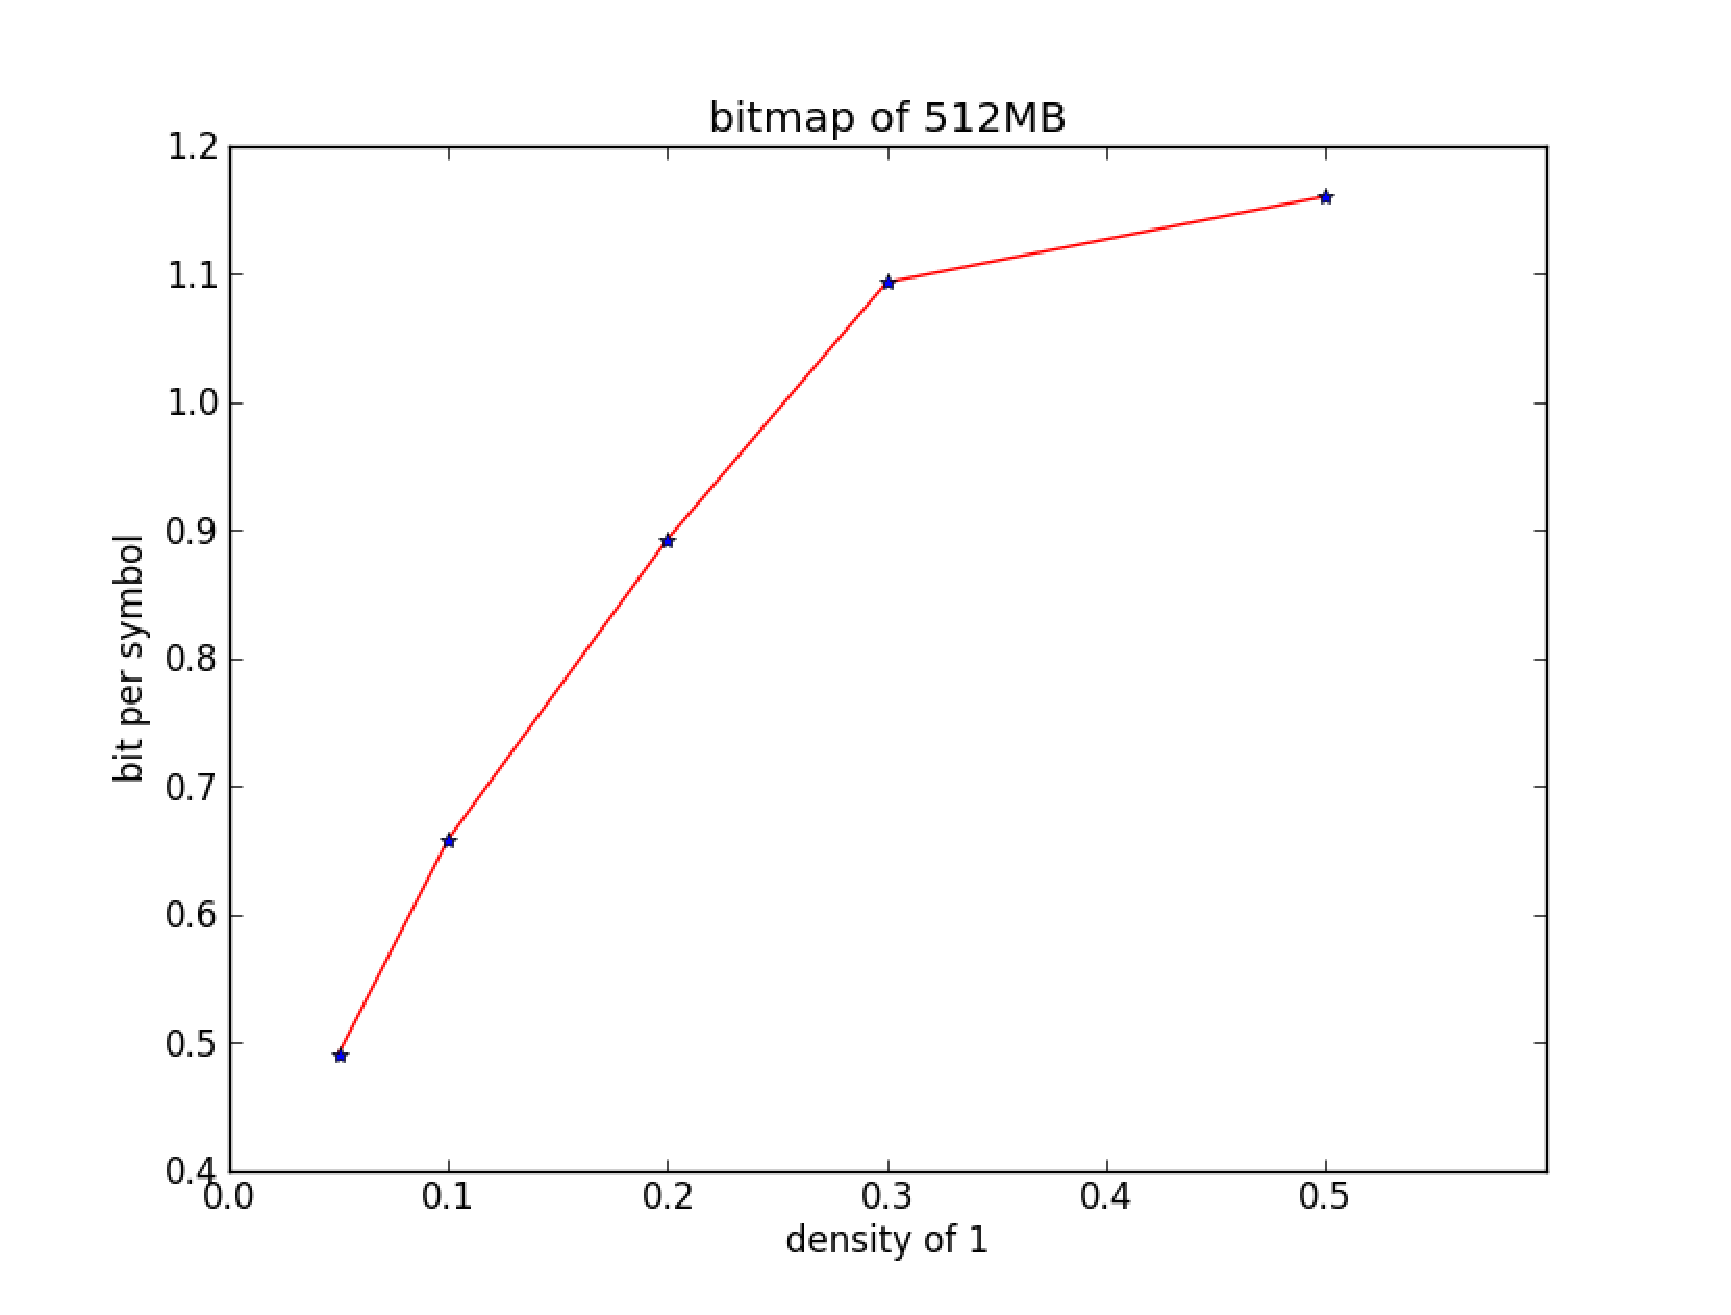
\includegraphics[width=0.8\textwidth]{rrr}
    \caption{RRR方法压缩率随序列经验熵的变化曲线}
\end{figure}


除了经典的RRR方法之外,近年来还出现了一些很有效的rank\&select数据结构实现\cite{okanohara2007practical},其中esp,recrank,vcode以及
sdarray都是类似于RRR方法,bit per symbol有可能达到小于1的实现。这些方法的性能表现在文献\cite{claude2009practical}和文
献\cite{okanohara2007practical}中都有详尽的叙述,这里只展示在空间占用上RRR方法和这几种方法的对比。

\begin{table}[htbp]
    \caption{RRR方法和其他几种方法的压缩效率对比}
    \label{tab:tabcom}
    \centering
    \begin{tabular}{lr}
    \toprule
    数据结构&Bit Per Symbol\\
    \midrule
    rrr&0.48\\
    sdarray&2.05\\
    recrank&1.25\\
    esp&0.50\\
    \bottomrule
    \end{tabular}
\end{table}

表\ref{tab:tabcom}中列出了几种方法和RRR方法的bit per symbol的大小对比,数据来源是论文\cite{claude2009practical},其测试数据是
500M的01序列,1的比例是5\%。在这一条件下,可以看到RRR方法具有明显的空间优势,其压缩率是最高的。

通过对RRR方法实现并和Jacobson的方法做实验对比,可知,在01序列并不均匀时,采用RRR方法具有明显的空间优势。而压缩后缀数组的
实现中所用得到的支持rank操作的字典则都是01序列不均匀分布的,所以在CSA中采用RRR方法实现rank操作会有更好的空间效果。Select操
作的实现是在rank的基础上实现的,总的时间复杂度可以看作rank操作的整数倍。在select操作相对于rank操作较少时,具有较好的表现。
RRR方式总体的效果是比较理想的,尤其是在空间占用上具有很大的优势,在实际应用中,若01序列的分布是很悬殊的,则RRR将是很可取的
一种rank\&select操作实现。

\section{压缩后缀数组和模式匹配}
\subsection{CSA前向搜索模式匹配算法}
从上一节对CSA性质的介绍中,我们知道后缀$T_{SA[\alpha(c)]},T_{SA[\alpha(c)+1]}\ldots T_{SA[\alpha(c)+\beta(c)-1]}$的首字符都
是$c$。设需要搜索的模式为$P[0\ldots m-1]$,首先对于字符$P[0]$,明显的其对应的在$T$中出现的位置为
$SA[\alpha(c)],SA[\alpha(c)+1]\ldots SA[\alpha(c)+\beta(c)-1]$,这个位置集可以表示为$SA[\alpha(c)\ldots\alpha(c)+\beta(c)-1]$,计为
$(l,r)$,称为后缀范围(suffix range)。下一步搜索$P[1]$,即检测$T[SA[\alpha(P[0])]+1],T[SA[\alpha(P[0])+1]+1],\cdots ,T[SA[\alpha(P[0])+\beta(P[0])-1]+1]$
是否等于$P[1]$。由后缀数组的性质可知,这一步的结果得到的后缀数组的下标依然是连续的。以此类推,直到模式串中最后一个字
符搜索完毕,即可得到匹配结果。

近一步观察上面的比较,可以发现,比较$T[SA[\alpha(P[0])]+1],T[SA[\alpha(P[0])+1]+1],\cdots ,T[SA[\alpha(P[0])+\beta(P[0])-1]+1]$
是否等于$P[1]$时并不需要比较字符串。因为$P[1]$对应的也有一个序列$SA[\alpha(P[1])],SA[\alpha(P[1])+1],\cdots ,SA[\alpha(P[1])+\beta(P[1])-1]$,所以只需要求出
$SA[\alpha(P[0])]+1,SA[\alpha(P[0])+1]+1,\cdots ,SA[\alpha(P[0])+\beta(P[0])-1]+1$和$SA[\alpha(P[1])],SA[\alpha(P[1])+1],\cdots ,SA[\alpha(P[1])+\beta(P[1])-1]$
的交集即为模式串$P[1]P[2]$出现的位置。

在上面的迭代过程中要求$SA[\alpha(P[0])]+1,SA[\alpha(P[0])+1]+1,\cdots ,SA[\alpha(P[0])+\beta(P[0])-1]+1$和$SA[\alpha(P[1])],SA[\alpha(P[1])+1],\cdots ,SA[\alpha(P[1])+\beta(P[1])-1]$的交集。
实际计算中无需求出相应的$SA$值,只需求出其对应后缀范围的交集即可,此时可以利用压缩后缀数组的性质$SA[i]+1=SA[\Phi[i]]$,
所以在计算中只需计算$\alpha(P[1]),\alpha(P[1])+1,\cdots , \alpha(P[1])+\beta(P[1])-1$和$\Phi[\alpha(P[0])],\Phi[\alpha(P[0])+1],\cdots , \Phi[\alpha(P[0])+\beta(P[0])-1]$
的交集即可。以此类推,可得到模式串$P$的后缀数组范围。

具体的算法描述如算法\ref{alg:forwardsearch}。

\begin{algorithm}
    \caption{前向搜索模式匹配}
    \label{alg:forwardsearch}
    \begin{algorithmic}[1]
        \Require $P,\Phi,\alpha,\beta$
        \Ensure $(l,r)$
        \Function{forwardSearch}{$P,\Phi,\alpha,\beta$}
        \State $m \gets size(P)$
        \State $n \gets size(CSA)$
        \State $(l,r) \gets (\alpha(P[0]),\alpha(P[0])+\beta(P[0])-1)$
        \For {$i \gets 1$ to $m-1$}
            \State $(l_{tmp},r_{tmp}) \gets (\alpha(P[i]),\alpha(P[i])+\beta(P[i])-1)$
            \For {$j \gets l$ to $r$}
            \If{$\Phi[j] \in (l_{tmp},r_{tmp})$}
                \State $l\gets j$
                \State break
            \EndIf
            \EndFor
            \For {$j \gets r$ down to $l$}
            \If{$\Phi[j] \in (l_{tmp},r_{tmp})$}
                \State $r\gets j$
                \State break
            \EndIf
            \EndFor
            \If{$l > r$}
                \State \Return $\varnothing$
            \EndIf
        \EndFor
        \State \Return $(l,r)$
        \EndFunction
    \end{algorithmic}
\end{algorithm}

算法\ref{alg:forwardsearch}的搜索过程和基于后缀数组的模式匹配算法是等价的。只是这里利用了$\Phi$数组的特性,总的时间复杂度
依然是$O(m\log n)$。

\subsection{CSA后向搜索模式匹配}
压缩后缀数组上的后向搜索模式匹配算法是由Sadakan最早提出来的\cite{sadakane2002succinct}。如上文中所述,我们用$(l,r)$
表示一个模式串在$T$上的后缀位置,模式匹配的目的正是要找到$P$的$(l,r)$。首先,计算$P[m]$的后缀位置,很明显$(\alpha(P[m]),
\alpha(P[m])+\beta(P[m])-1)$就是。假设一般情况,我们已经知道$P[i+1\ldots m-1]$的后缀数组位置为$(l_{P_{i+1}},r_{P_{i+1}})$,
那么$P[i\ldots,m-1]$的后缀数组位置$(l_{P_i},r_{P_i})$必定是由$P[i]$的后缀数组位置的一部分组成的,设$P[i]$的后缀数组位置
为$(l_{P[i]},r_{P_i})$,那么对于$l_{P[i]\leq k \leq r_{P_i}}$只要$SA^{-1}SA[k]+1$在$(l_{P_{i+1}},r_{P_{i+1}})$中,$k$一定在$(l_{P_i},r_{P_i})$
中。也就是说$P[i\ldots n-1]$的出现位置一定是$P[i]$的出现位置后面紧跟着$P[i+1\ldots m-1]$的出现位置。加上$\Phi[i]=SA^{-1}[SA[i]+1]$,
所以我们可以得到公式\ref{equa:equa1}。

\begin{equation}\label{equa:equa1}
    k \in (l_{P_i},r_{P_i}) \iff k \in (l_{P[i]},r_{P[i]}) \wedge \Phi[k] \in (l_{P_{i+1}},r_{P_{i+1}})
\end{equation}

由于在简明数据结构存储下$\Phi$可以在常数时间内获得,并且其值在$(l_{P_{i+1}},r_{P_{i+1}})$上是递增的,所以,可以用二分搜索
来搜索$\Phi[k]$是否在$(l_{P_{i+1}},r_{P_{i+1}})$上,时间复杂度是$O(\log n)$。重复上述过程$m$次,即可在CSA上用$O(m\log n)$
时间复杂度找到模式$P[0\ldots m-1]$的后缀数组范围$(l,r)$

算法\ref{alg:backwardsearch}给出了CSA上的后向搜索的伪代码。而图\ref{figbackwardsearch}给出了一个采用算法\ref{alg:backwardsearch}
的例子,搜索模式$P=CCAGTA$。每一个方块儿对应一个字符的后缀数组区域,灰色的区域表示对应$P$的一个后缀在$T$的后缀数组上的位置
范围。在右起第二步,计算新的区域时,根据下一个字符$G$的后缀范围,计算其$\Phi$值,查看这个$\Phi$是否落在当前模式$TA$的后缀范
围内,由于$\Phi$的递增特性,很容易用二分搜索方法找到新的区域的上下界。

\begin{algorithm}
    \caption{后向搜索}
    \label{alg:backwardsearch}
    \begin{algorithmic}[1]
        \Require $P,\Phi,\alpha,\beta$
        \Ensure $(l,r)$
        \Function{backwardSearch}{$P,\Phi,\alpha,\beta$}
        \State $l_{m} \gets 0;r_{m}\gets n-1$
        \For {$i\gets m-1$ down to $0$}
            \State $l_i \gets \min\{ k \in [\alpha(P[i]),\alpha(P[i])+\beta(P[i])-1],\Phi[k] \in [l_{i+1},r_{i+1}]\}$
            \State $r_i \gets \max\{ k \in [\alpha(P[i]),\alpha(P[i])+\beta(P[i])-1],\Phi[k] \in [l_{i+1},r_{i+1}]\}$
            \If{$l> r$}
                \State \Return $\varnothing$
            \EndIf
        \EndFor
        \State \Return $(l_0,r_0)$
        \EndFunction
    \end{algorithmic}
\end{algorithm}


\begin{figure}[t]
    \centering
    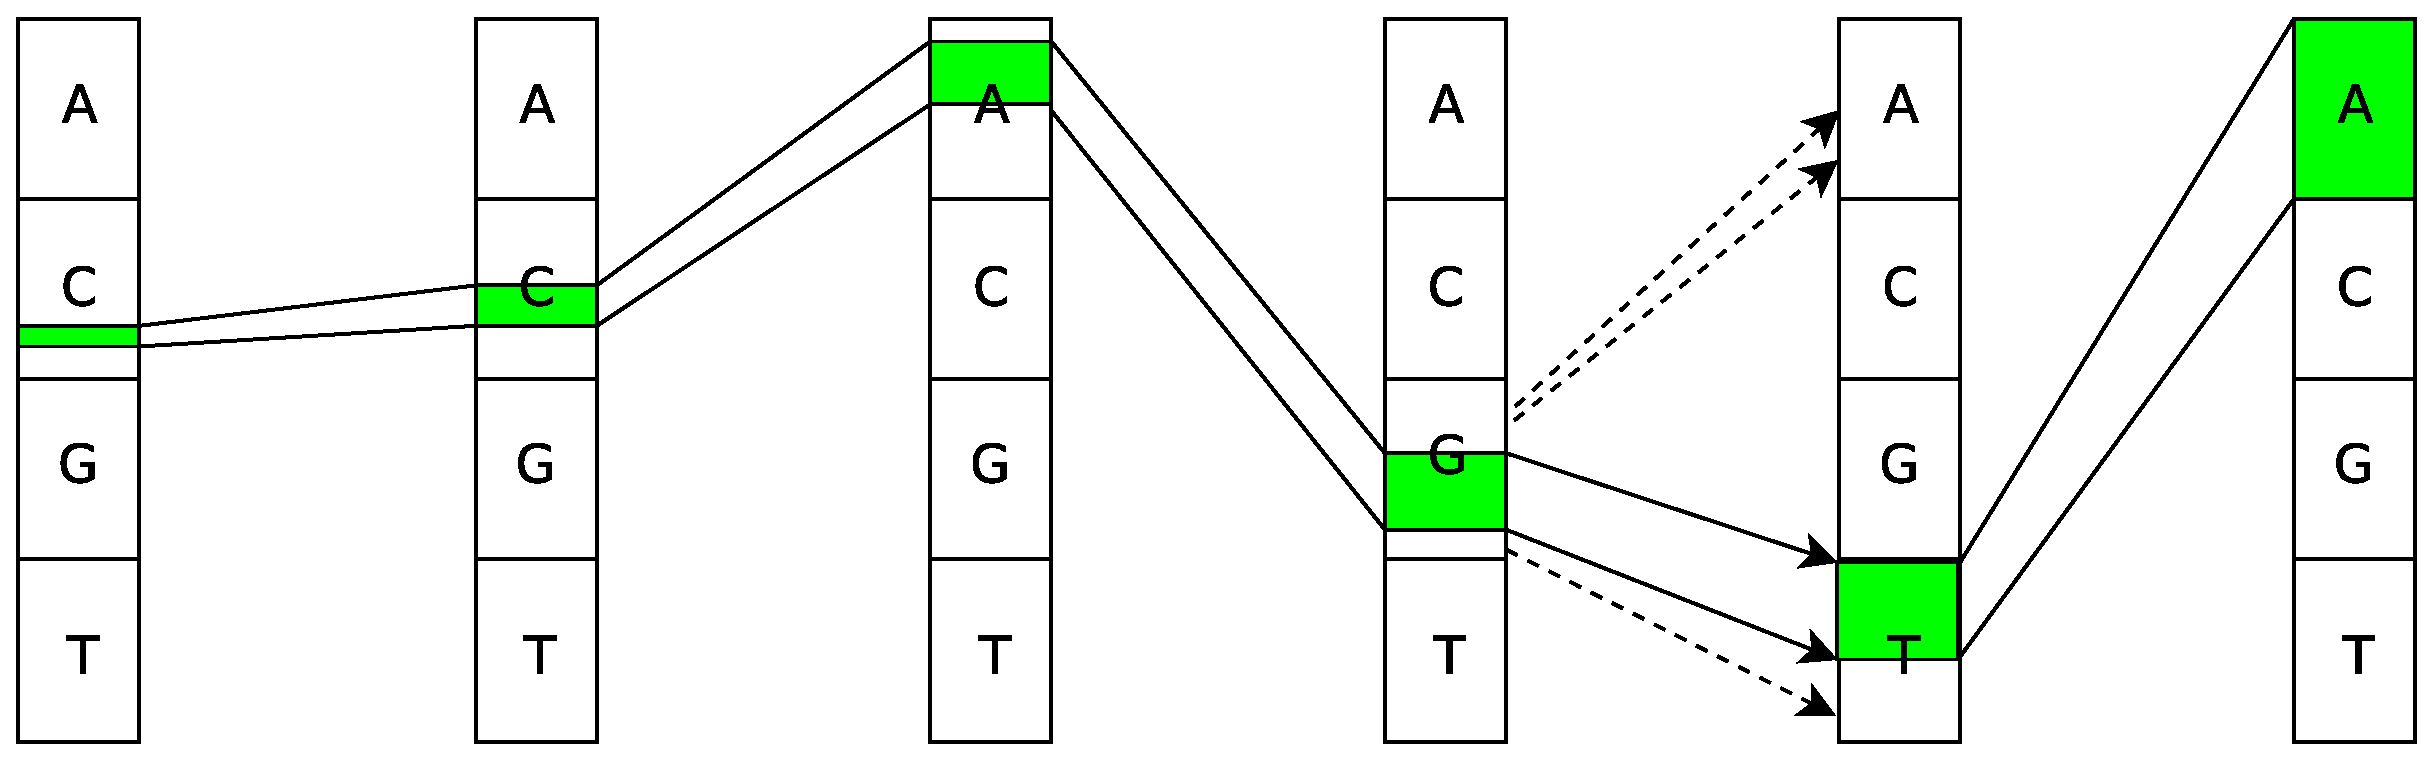
\includegraphics[width=0.7\textwidth]{csa_backwardsearch}
    \caption{CSA上的后向搜索}
    \label{figbackwardsearch}
\end{figure}

\section{压缩后缀数组和自索引}
压缩后缀数组优于后缀数组的另一性质是其自索引性。在上一小节的模式匹配算法中,可以看到并不需要原文本$T$即可完成匹配,
基于这个原理,只要给压缩后缀数组添加一个辅助数组即可实现压缩后缀数组的自索引算法。

考虑已知$\Sigma$中任意字符$c$的$\alpha(c)$值,则$\beta(c)=\alpha(c+1)-\alpha(c)$,所以只需保存$\alpha(c)$即可完成
无需原文本的模式匹配,基于此在压缩后缀数组基础上增加一个辅助数组$\alpha$即可实现自索引。

考虑下面的性质$T[SA[\alpha(c)]]=T[SA[\alpha(c)+1]]=\cdots=T[SA[\alpha(c)+\beta(c)-1]]=c$,所以对于$T$中任意位置$i$处
的字符,只要求出其对应后缀$T_i$的名次,即$j=SA^{-1}[i]$,便可在$\alpha$数组中搜索其所在区间使得对某个字符$c$存
在$\alpha(c)\leq j< \alpha(c+1)$,即得到$T[SA[j]]=c$,所以即可知$T[i]=c$。而由前文中可所述$\Phi$的性质可知后缀数组的
逆数组$SA^{-1}$是可以在线性时间内得到的。

按照上面叙述的方法可以很方便的恢复出文本$T$的任意字符,进而恢复出$T$的任意长的子串$T_{i,j}$。在实际运算中
考虑到压缩后缀数组的性质$SA^{-1}[i+1]=\Phi[SA^{-1}[i]]$,所以在已知$SA_[i]$求出$T[i]$的情况下求$T[i+1]$时,
不必再求$SA^{-1}[i+1]$,直接返回$\Phi[SA^{-1}[i]]$,这个计算是常数时间的,而不是线性时间\cite{sadakane2000compressed}。

具体算法如算法\ref{alg:getT}。

\begin{algorithm}
    \caption{CSA自索引}
    \label{alg:getT}
    \begin{algorithmic}[1]
        \Require $\Phi,\alpha,i,j$
        \Ensure $T[i\ldots j]$
        \For {$k\gets i$ to $j$}
            \If {k=i}
                \State $rank \gets SA^{-1}[k]$
                \State $prev \gets rank$
            \Else
                \State $rank \gets \Phi[prev]$
            \EndIf
            \State $T[k] \gets$ \Call{binarySearch}{$rank$,$\alpha$}
        \EndFor
        \State \Return $T[i\ldots j]$
    \end{algorithmic}
\end{algorithm}

上述算法总共执行$m=j-i+1$步,每一步执行一次$|\Sigma|$上的二分搜索,且要求$SA$,所以时间复杂度为
$O(\log |\Sigma|+\log \log n)$,所以总的时间复杂度为$O(m(\log |\Sigma|+\log \log n))$。

\section{本章小结}
本章主要在前面阐述的后缀数组和压缩后缀数组性质的基础上提出了基于压缩后缀数组的文本索引和自索引算法。并详细介绍了上实现压缩
后缀数组的基本数据结构:RRR算法。之后介绍了两种CSA上的$O(m\log n)$时间复杂度的模式匹配算法:前向搜索和后向搜索。为下一章的
DNA序列比对算法给出实现基础。最后还介绍了CSA的自索引性质,并给了由压缩后缀数组恢复原文本序列的算法。
